\documentclass{article}
\usepackage[margin=1in]{geometry}
\usepackage{amsmath}
\usepackage{graphicx}
\usepackage{float}
\usepackage{listings}
\usepackage{xcolor}

\lstset{
    language=Matlab,
    basicstyle=\ttfamily\footnotesize,
    keywordstyle=\color{blue},
    breaklines=true
}

\begin{document}

\section*{Problem 1(a)}

Consider the steady-state advection-diffusion problem on $\Omega = [0,1]$:
\begin{equation}
    c u_x = \nu u_{xx} + f
\end{equation}
with boundary conditions $u(0) = u(1) = 0$. The parameters are $L=1$, $c=1$, $\nu=10^{-3}$, and $f=1$.

\subsection*{Analytical Solution}
The exact analytical solution is required to compute the pointwise relative error. The general solution is:
\begin{equation}
    u(x) = C_1 + C_2 e^{\frac{c}{\nu}x} + \frac{f}{c}x
\end{equation}
Applying the Dirichlet boundary conditions yields:
\begin{equation}
    u(x) = \frac{f}{c} \left( x - \frac{e^{\frac{c}{\nu}x} - 1}{e^{\frac{c}{\nu}L} - 1} \right)
\end{equation}
To avoid floating-point overflow during computation ($\frac{c}{\nu} = 1000$), the exact solution is approximated by the stable boundary layer form:
\begin{equation}
    u(x) \approx x - e^{\frac{c}{\nu}(x - 1)}
\end{equation}

\subsection*{Finite Element Formulation}
The domain is discretized into $E=100$ uniform elements with $h_e = 0.01$. Linear basis functions are utilized. The element matrices are:
\begin{equation}
    A^e = \frac{1}{h_e} \begin{bmatrix} 1 & -1 \\ -1 & 1 \end{bmatrix}, \quad
    C^e = \frac{1}{2} \begin{bmatrix} -1 & 1 \\ -1 & 1 \end{bmatrix}, \quad
    F^e = \frac{f h_e}{2} \begin{bmatrix} 1 \\ 1 \end{bmatrix}
\end{equation}
The global system $( \nu A + c C ) \underline{u} = F$ is assembled and solved after applying the boundary conditions.

\subsection*{Results}
The local element P\'eclet number is $Pe = \frac{c h_e}{2\nu} = 5$. Because $Pe > 1$, the standard Galerkin formulation exhibits severe non-physical spatial oscillations near the right boundary ($x=1$). 

The computed maximum pointwise relative error is \textbf{0.6735}.

\begin{figure}[H]
    \centering
    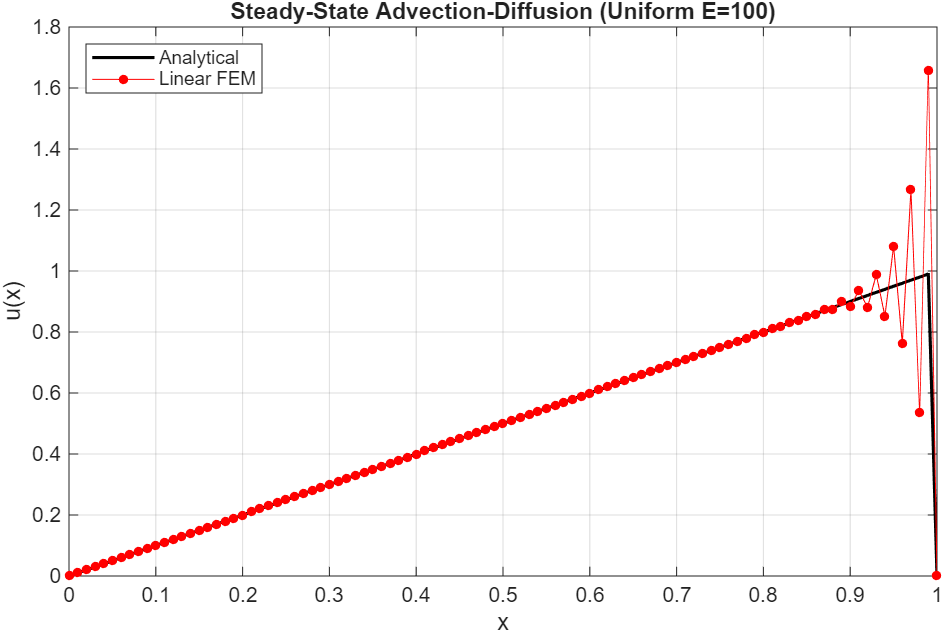
\includegraphics[width=0.7\textwidth]{1_a.png}
    \caption{Steady-State Advection-Diffusion using a uniform mesh ($E=100$).}
    \label{fig:1a}
\end{figure}

\subsection*{MATLAB Implementation}
\begin{lstlisting}
L = 1.0; c = 1.0; nu = 1e-3; f = 1.0;
E = 100; N = E + 1; h = L / E;

x = linspace(0, L, N)';
K = sparse(N, N);
F = zeros(N, 1);

for e = 1:E
    A_e = (1.0 / h) * [1.0, -1.0; -1.0, 1.0];
    C_e = 0.5 * [-1.0, 1.0; -1.0, 1.0];
    idx = [e, e+1];
    K(idx, idx) = K(idx, idx) + nu * A_e + c * C_e;
    F(idx) = F(idx) + (f * h / 2.0) * [1.0; 1.0];
end

K(1, :) = 0.0; K(1, 1) = 1.0; F(1) = 0.0;
K(end, :) = 0.0; K(end, end) = 1.0; F(end) = 0.0;

u_h = K \ F;

u_ex = x - exp((c / nu) * (x - L));
u_ex(1) = 0.0; u_ex(end) = 0.0;

interior_idx = 2:(N-1);
rel_error = max(abs(u_ex(interior_idx) - u_h(interior_idx)) ./ abs(u_ex(interior_idx)));
fprintf('Maximum pointwise relative error: %.4e\n', rel_error);
\end{lstlisting}

\end{document}